
\documentclass{beamer}

\usepackage[utf8]{inputenc}
\usetheme{Warsaw}

%Information to be included in the title page:
\title{MTH 201: Calculus}
\subtitle{Module 1B: The concept of the limit (AC 1.2)}
\author{Prof. Talbert}
\institute{GVSU}
\date{\today}


\begin{document}

\frame{\titlepage}


\begin{frame}{Agenda for today}
    \begin{itemize}
        \item<1-> Review of Daily Prep assignment, and Q+A
        \item<2-> Activity: Finding limits with algebra 
        \item<3-> Activity: Instantaneous velocity again 
        \item<4-> Further practice with the concept
        \item<5-> For next time: Followup activities and things to do 
    \end{itemize}
\end{frame}

\begin{frame}{Polling for today}
    \large{
    Go to \textbf{\url{www.mentimeter.com}} and enter code \texttt{xx yy zz} 
    }
    \end{frame}

\begin{frame}{Finding limits using algebra}
      \begin{alertblock}{Alert}
        \textbf{Finding a limit of a function at a point, is not always the same thing as evaluating the function at that point.}
      \end{alertblock}
      
     \begin{exampleblock}{Example}
     \begin{equation*}
         \lim_{x \to 2} \frac{x^2-4}{x-2} = 4
     \end{equation*}
    \begin{center}
             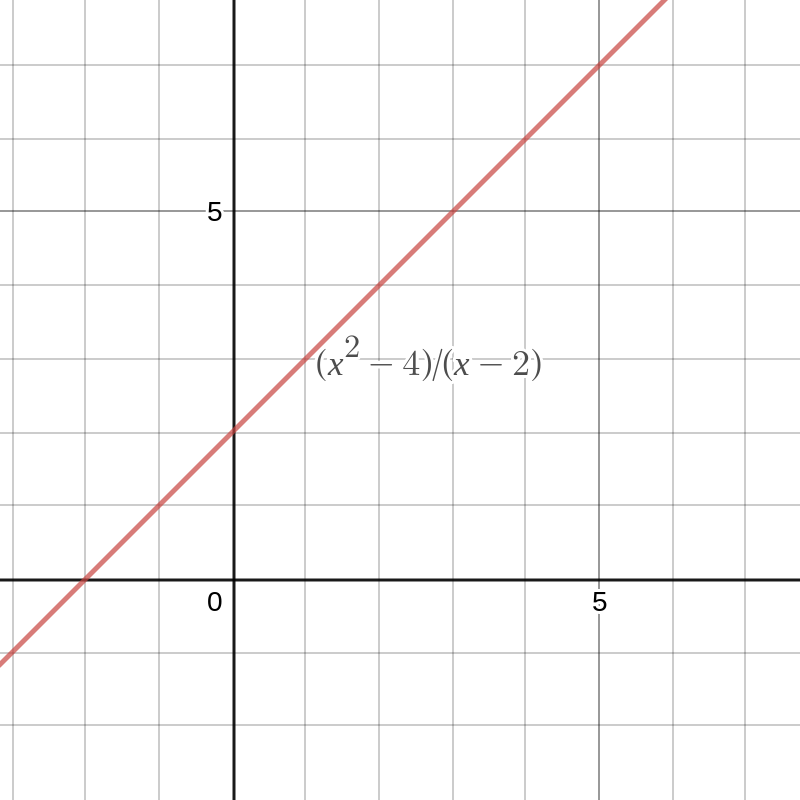
\includegraphics[width=1.25in]{1b-in-1.png}
    \end{center}
         But $\frac{x^2 - 4}{x-2}$ evaluated at $x=2$ is undefined ($0/0$). 
     \end{exampleblock}
\end{frame}

\begin{frame}{Using algebra first}
    \begin{block}{Pro Tip}
    Always try to simplify the algebra first. 
    \end{block}
    
    \begin{exampleblock}{Example}
     \begin{align*}
         \lim_{x \to 2} \frac{x^2-4}{x-2} &= \lim_{x \to 2} \frac{(x-2)(x+2)}{x-2} \\
         &= \lim_{x \to 2} (x+2)
     \end{align*}
    As $x$ gets closer to $2$, $x+2$ gets closer to $4$. \vskip
    
    Therefore $\lim_{x \to 2} \frac{x^2-4}{x-2} = 4$.
        \end{exampleblock}
\end{frame}

\begin{frame}{Practice with the concept}
    
    Go to: 
    
    \begin{center}
        \url{http://gvsu.edu/s/1pq}
    \end{center}
    
Find the value of the limit using algebra simplification first. 

\begin{itemize}
    \item $(x+2)^3$ does not equal $x^3 + 8$
    \item The answer is 12. 
\end{itemize}
    
\end{frame}

\begin{frame}{Average velocity}

    Consider a moving object whose position function is given by $s(t) = t^2$ where $t$ is time in seconds, $s$ is position in meters. 
    
    \begin{center}
        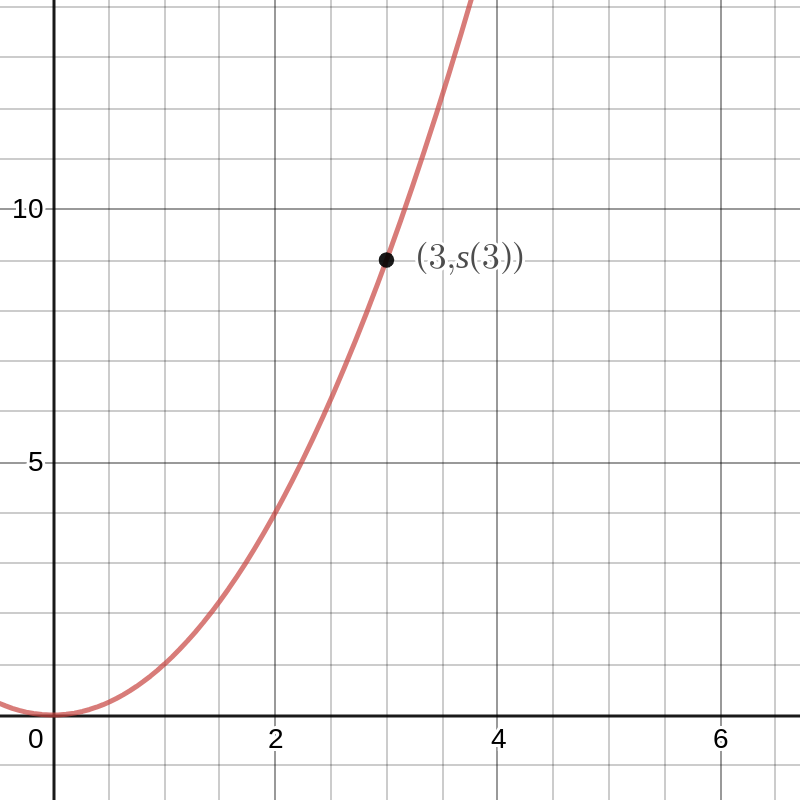
\includegraphics[width=2in]{1b-in-2.png}
    \end{center}
    
    \end{frame}
    
    \begin{frame}{Finding average and instantaneous velocity}
    
    The \textbf{average velocity} on the small time interval from $t=3$ to $t=3+h$ is
    \begin{equation*}
        \frac{s(3+h)-s(3)}{(3+h)-3} = \frac{s(3+h) - s(3)}{h}
    \end{equation*}
    
    On Mentimeter: If we wanted to find the \textit{instantaneous velocity} at $t=3$, how would we modify this? 
        
    \end{frame}
    
    \begin{frame}{Working out the velocity}
        We get the instantaneous velocity at $t=3$ by taking the \textbf{average velocity} expression and \textbf{evaluating its limit as $h \to 0$}: 
        
        \begin{equation*}
            IV_{t=3} = \lim_{h \to 0} \frac{s(3+h) - s(3)}{h}
        \end{equation*}
        
    But we can now work out the value with algebra! Work with your partner to do this: 
        \begin{center}
            \url{http://gvsu.edu/s/1pt}
        \end{center}
    
    Spoiler: The answer is 6 meters/second. 
    \end{frame}
    
    \begin{frame}{Getting the instantaneous velocity}
    \begin{align*}
        IV_{t=3} &= \lim_{h \to 0} \frac{s(3+h) - s(3)}{h} \ \text{Setup} \\
        &= \lim_{h \to 0} \frac{(3+h)^2 - 9}{h}  \ \text{Apply formula} \\
        &= \lim_{h \to 0} \frac{9 + 6h + h^2 - 9}{h}  \ \text{FOIL} \\
        &= \lim_{h \to 0} \frac{6h + h^2}{h}  \ \text{Subtract 9s} \\
        &= \lim_{h \to 0} \frac{h(6 + h)}{h}  \ \text{Factor out} \\
        &= \lim_{h \to 0} (6+h)  \ \text{Divide off factor} \\
        &= 6 \ \text{meters/second}  \ \text{Let $h$ go to $0$}
    \end{align*}
    
    \end{frame}


\begin{frame}
    \frametitle{NEXT TIME...}

    \begin{itemize}
        \item To do list 1
        \item To do list 2
    \end{itemize}

\end{frame}

\end{document}